% Created on Oct 2023 by Mohammad Bashiri

\documentclass[twoside, 12pt, a4paper]{report}

% If you want to print the document set the argument to "print", otherwise to "online". Default: "online"
%   - "print": adjusts the margins such that when printed the two side-by-side pages have similar outer margin
%   - "online": same margin for all pages
\usepackage[print]{preambles}

%% If this is a draft, you can specifically show that by uncommenting the lines below
% \usepackage{draftwatermark}
% \SetWatermarkText{DRAFT}
% \SetWatermarkScale{5}
% \SetWatermarkAngle{60}
% \SetWatermarkColor[gray]{0.95}

% font sizes:
% \tiny
% \scriptsize
% \footnotesize
% \small
% \normalsize
% \large
% \Large
% \LARGE
% \huge
% \Huge

\begin{document}
\def\biblio{}

\pagenumbering{gobble}
\begin{titlepage}
    \begin{center}
        \vspace*{1cm}
        
        \Huge\textbf{Your Thesis Title}
        
        \vspace{5.5cm}
        
        \large\textbf{Dissertation}\\
        der Mathematisch-Naturwissenschaftlichen Fakultät\\
        der Eberhard Karls Universität Tübingen\\
        zur Erlangung des Grades eines\\
        Doktors der Naturwissenschaften\\
        (Dr. rer. nat.)
        
        \vspace{6.0cm}
        
        vorgelegt von\\
        First Last\\
        aus City, Country\\
        
        \vspace{2.2cm}
        
        Tübingen\\
        20XX
        
    \end{center}
\end{titlepage}

\newpage 
\ % The empty page

\newpage
\vspace*{\fill}
Gedruckt mit Genehmigung der Mathematisch-Naturwissenschaftlichen Fakultät der Eberhard Karls Universität Tübingen. \\ \\ \\
Tag der mündlichen Qualifikation: \tab TBD \\ \\%01.12.2023 \\ \\
Dekan: \tab Prof. Dr. First Last \\
1. Berichterstatter: \tab Prof. Dr. First Last \\
2. Berichterstatter: \tab Prof. Dr. First Last

\newpage 
\ % The empty page

\newpage
\vspace*{\fill}
Ich erkläre, dass ich die zur Promotion eingereichte Arbeit mit dem Titel “Latent Variable and Implicit Models for Neural System Identification” selbstständig verfasst, nur die angegebenen Quellen und Hilfsmittel benutzt und wörtlich oder inhaltlich übernommene Stellen als solche gekennzeichnet habe. Ich versichere an Eides statt, dass diese Angaben wahr sind und dass ich nichts verschwiegen habe. Mir ist bekannt, dass die falsche Abgabe einer Versicherung an Eides statt mit Freiheitsstrafe bis zu drei Jahren oder mit Geldstrafe bestraft wird. 

\begingroup
  \centering
  \wildcard{Ort/Place, Datum/Date}
  \hspace{1cm}
  \wildcard{Unterschrift/Signature}
  \par
\endgroup

\newpage 
\ % The empty page

\chapter*{Acknowledgements}
\label{ch:ack}
% \addcontentsline{toc}{chapter}{\nameref{ch:ack}}
\lipsum[2-4]

\newpage 
\ % The empty page

\chapter*{Abstract}
\label{ch:abstract}
% \addcontentsline{toc}{chapter}{\nameref{ch:abstract}}
\lipsum[2-4]

\newpage 
\ % The empty page

\chapter*{Zusammenfassung}
\label{ch:zusammenfassung}
% \addcontentsline{toc}{chapter}{\nameref{ch:zusammenfassung}}
\lipsum[2-4]

\newpage 
\ % The empty page

\newpage
\pagenumbering{arabic}
\setcounter{page}{6}
\tableofcontents

\subfile{chapters/1.introduction}
\subfile{chapters/2.background}
\subfile{chapters/3.paper}
\subfile{chapters/6.discussion}

\newpage
\bibliographystyle{unsrtnat}
\bibliography{references}

\addtocontents{toc}{\protect\setcounter{tocdepth}{0}}
% From this point on, only show up to \chapters in the ToC

\chapter*{Appendix}
\addcontentsline{toc}{chapter}{Appendices}
\renewcommand{\thesection}{Manuscript \arabic{section}}

This chapter contains the publications discussed in chapters X-Y.

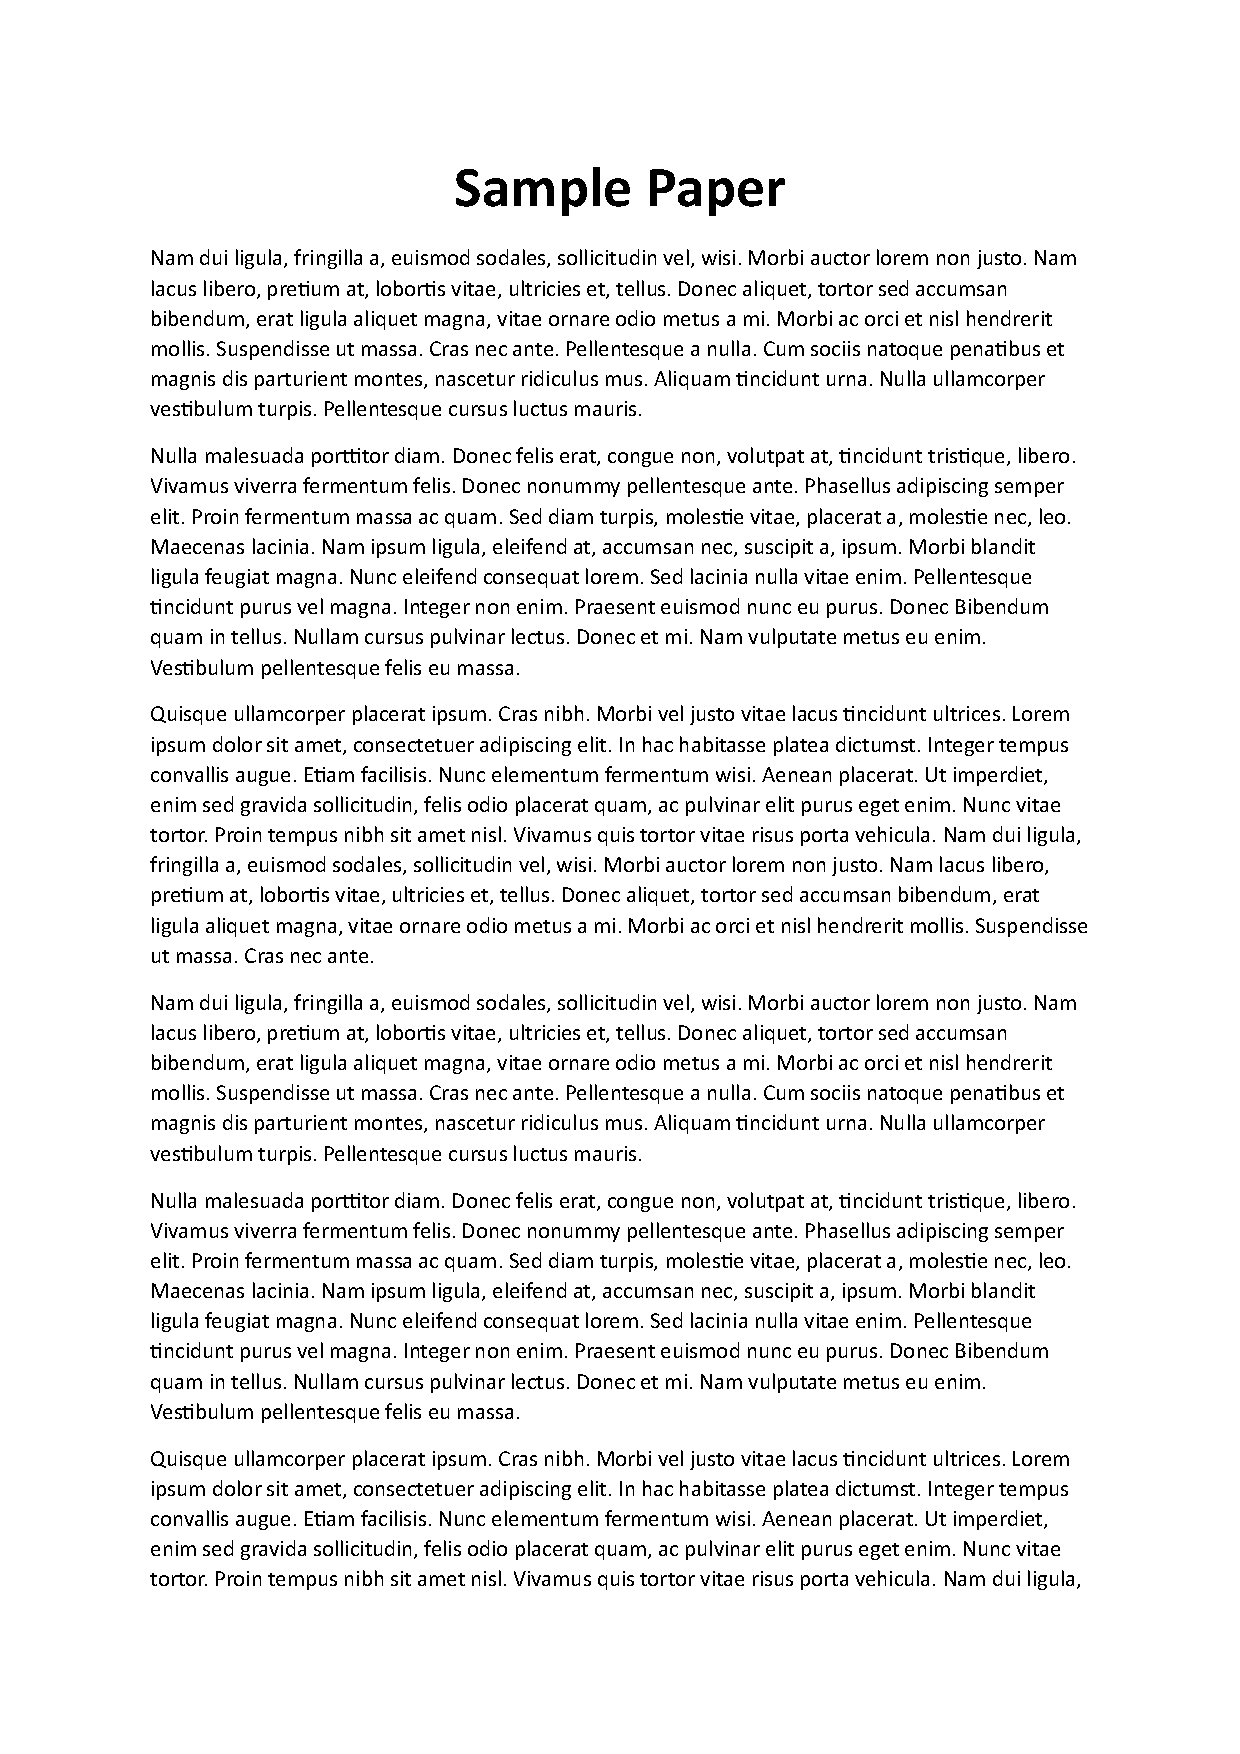
\includepdf[
    pages=1,
    trim=18mm 12mm 18mm 20mm, % left bottom right top
    scale=.82,
    frame,
    pagecommand={\section{}\label{paper:paper}},
    linktodoc=true]
    {manuscripts/paper.pdf}
\includepdf[
    pages=2-,
    trim=18mm 12mm 18mm 20mm,
    scale=.82,
    frame,
    pagecommand={},
    linktodoc=true]
    {manuscripts/paper.pdf}

\end{document}
